% ======================================================================
\section{Diseño de la interfaz de usuario}
En esta sección se describe el diseño de la interfaz del usuario a partir del análisis llevado a cabo.

El intérprete presenta una interfaz de consola de comandos, por lo que el diseño se corresponde con una descripción de los usos 
del comando y el listado de las opciones que acepta.

El cliente runTree y la web en general presenta una interfaz web. El diseño se corresponde con una descripción 
gráfica de las páginas que la conforman y de las secciones que las componen.
% ======================================================================
\subsection{Intérprete}
El intérprete es un programa de consola de comando por lo que la interfaz con el usuario no es gráfica.

El comando ``omi'' permite ejecutar el intérprete. Se puede usar de las siguientes forma:
\begin{itemize}
   \item omi [opciones] $<fichero>$ [argumentos...]
   \item omi -c $<codigo>$ [argumentos...]
   \item omi -i [argumentos...]
   \item omi -sj $<fichero.json>$
\end{itemize}

El listado de opciones que acepta el comando a continuación:

\begin{description}
\item[-i	]:	Ejecuta el intérprete de forma interactiva.
 \item [-c $<codigo>$]:	Interpreta el código dado.
 \item [-l $<fichero.so>$]: Carga el módulo $<fichero.so>$.
\item [-h]: Muestra la ayuda.
 \item[-V]: Muestra la versión.
\item [-j $<fichero.json>$]: Imprime una descripción del procesos en formato json en el fichero $<fichero.json>$.
  \item [-x $<pasos>$]: Obtiene $<pasos>$ pasos del proceso de interpretación en cada petición. 
 \item [-s]:	Ejecuta como servidor en el puerto 8888.
\end {description}

% ======================================================================
\subsection{runTree}

runTree es un cliente web del intérprete OMI. Muestra información sobre el proceso de interpretación y permite navegar por este. 

El sistema lo compone una única página web con un diseño de cuadrícula.

\begin{center}
\includegraphics[scale=0.2]{runtree.png} \\
\end{center}

La primera parte de la retícula, superior izquierda, muestra el árbol sintáctico correspondiente al código enviado. En este árbol se marcarán los nodos a medida 
que se van ejecutando y resolviendo semánticamente. Además mostrará información directa de cada nodo tal como el nombre, el valor o el tipo.

En la segunda parte, superior derecha, muestra las tablas de símbolos de variables, funciones y clases. Esta sección permite navegar por las tablas de símbolos 
y los elementos que serán referenciados desde las mismas.

En la tercera parte, inferior izquierda, se muestra el código fuente y la interfaz de entrada/salida del programa.

En la última sección, inferior derecha, se muestra una consola informativa, en la que aparece una descripción del nodo actualmente en ejecución o 
los nodos seleccionados por el usuario. También se colocan en esta sección las opciones de control para avanzar un paso, una sentencia, la reproducción automática, abrir un fichero local o guardar el 
código en un fichero local. 

\subsection{Sitio web}
Según el análisis de la interfaz de usuario llevado a cabo se procede a detallar gráficamente cada página descrita.

\subsubsection{Home}
\begin{center}
\includegraphics[scale=0.2]{home.png} \\
\end{center}

\subsubsection{Sobre OMI}
\begin{center}
\includegraphics[scale=0.2]{about.png} \\
\end{center}

\subsubsection{Contacto}
\begin{center}
\includegraphics[scale=0.2]{contact.png} \\
\end{center}

\subsubsection{Índice de la documentación}
\begin{center}
\includegraphics[scale=0.2]{doc-index.png} \\
\end{center}

\subsubsection{Documento}
\begin{center}
\includegraphics[scale=0.2]{doc-content-x.png} \\
\end{center}

\subsubsection{Navegador de gramática}
\begin{center}
\includegraphics[scale=0.2]{gramatic-x.png} \\
\end{center}

\subsubsection{Navegador de clases}
\begin{center}
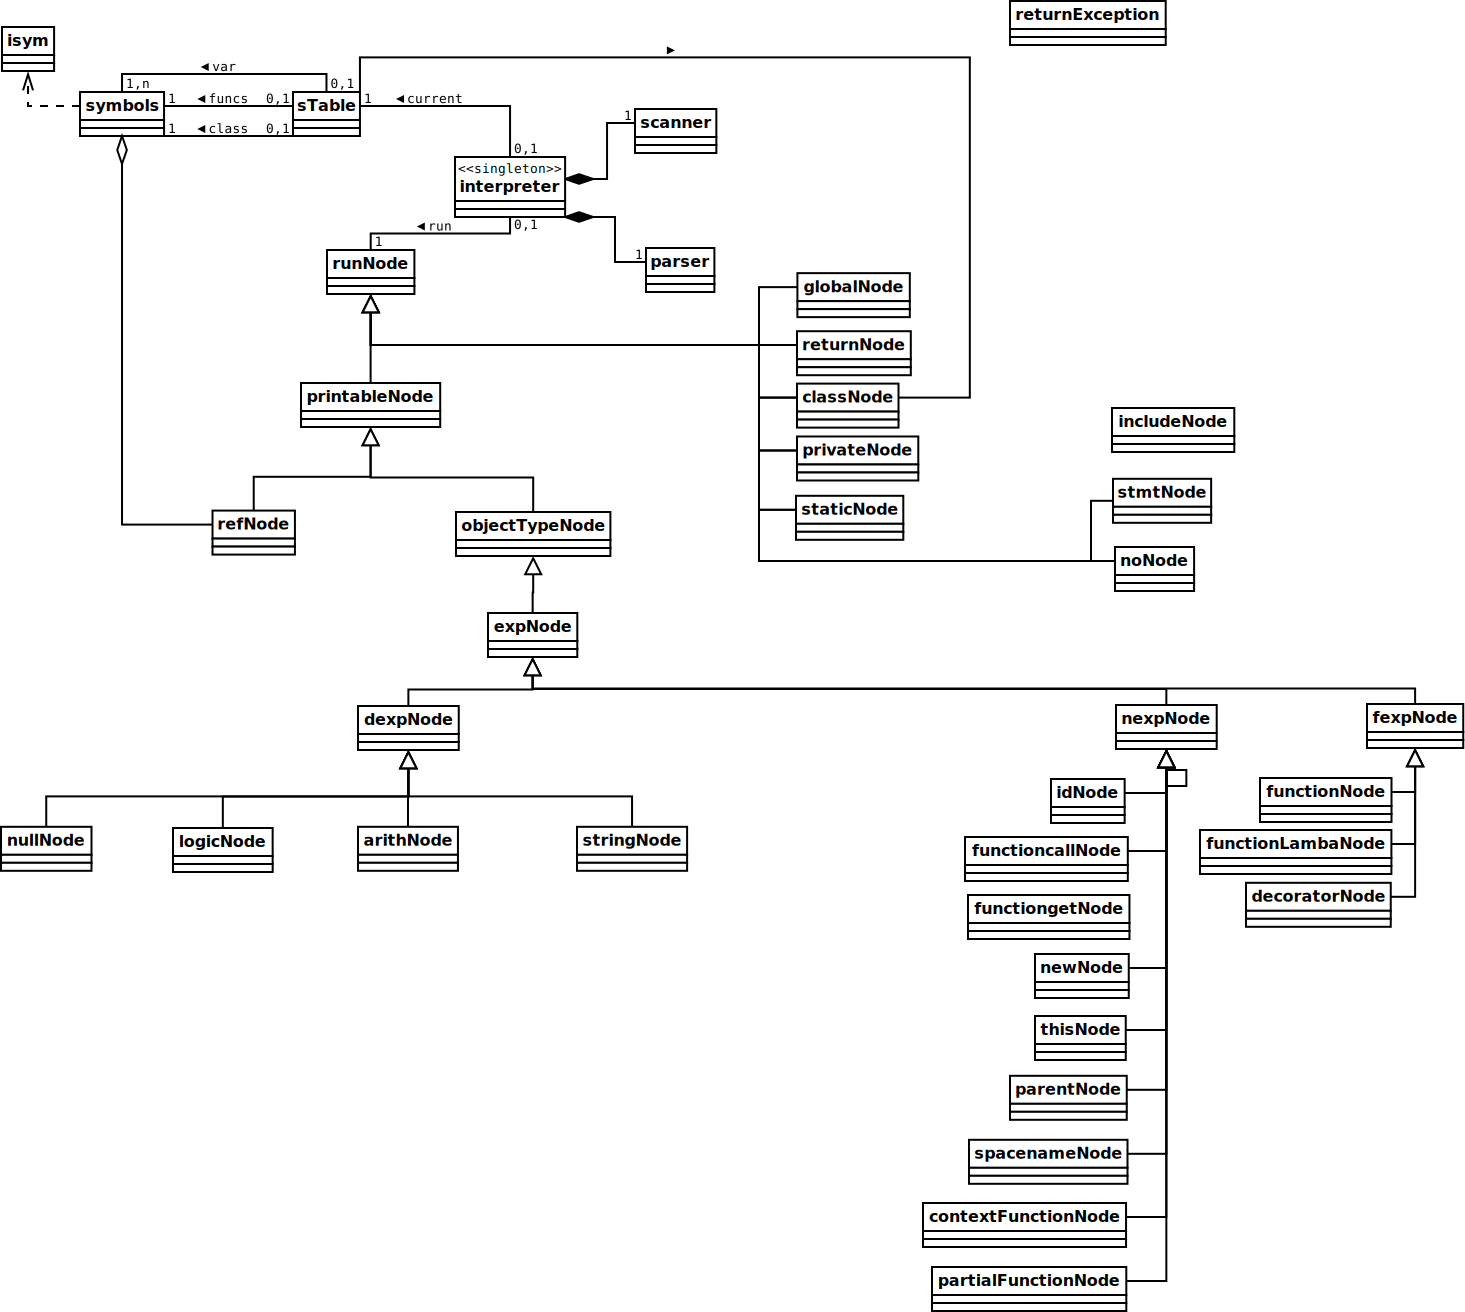
\includegraphics[scale=0.2]{class.png} \\
\end{center}

\subsubsection{Navegador de ficheros}
\begin{center}
\includegraphics[scale=0.2]{files.png} \\
\end{center}

\subsubsection{Descargas}
\begin{center}
\includegraphics[scale=0.2]{download.png} \\
\end{center}
